
\documentclass{standalone}

%\documentclass[convert]{standalone}
% convert: in addition to pdf output files, png files are created
% convert options does work properly with -output-directory option of latexmk

\usepackage{tikz-feynman}
\tikzfeynmanset{compat=1.1.0}


\begin{document}
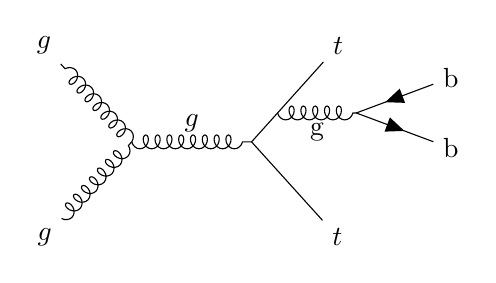
\begin{tikzpicture}
          \begin{feynman}
            \diagram [horizontal=a to b] {
            % draw s-channel gg->ttbar as usual
              i1 [particle=\(g\)]
                -- [gluon] a
                -- [gluon] i2 [particle=\(g\)],
              a -- [gluon, edge label=\(g\)] b,
              f1 [particle=\(t\)]
                -- b
                --  f2 [particle=\(t\)]],
            };

            % add vertex for FSR at 0.3 between vertex (b) and (f1)
            % add end vertex for FSR (with label H), then draw line between FSR vertices
            \vertex at ($(b)!0.3!(f1)$) (fsr_start);
            \vertex [right=1cm of fsr_start] (fsr_end);
            \draw [gluon] (fsr_start) -- node[below] {g} (fsr_end);

            % adds bbar
            \vertex [right=1.2cm of fsr_end] (b12_invis_helper);    % helper
            \vertex [above=0.2cm of b12_invis_helper] (b1) {b};
            \vertex [below=0.2cm of b12_invis_helper] (b2) {b};
            \draw [fermion] (b1) -- (fsr_end);
            \draw [fermion] (fsr_end) -- (b2);

            % adds bbar decay -alternative
            % \vertex [above right=of fsr_end] (b1) {b};
            % \vertex [below right=of fsr_end] (b2) {b};
            % \draw [fermion] (fsr_end) -- (b1);
            % \draw [fermion] (b2) -- (fsr_end);
          \end{feynman}
        \end{tikzpicture}
\end{document}
